\documentclass{picocon-fanzine}
\usepackage{xcolor}
\usepackage{soul}
\usepackage{array}
\usepackage{textgreek}
\usepackage{pgfplots}
\usepackage{pgfplotstable}
\usepackage{xcolor}
\usepackage{soul}
\usepackage{amsmath}
\usepackage{pdfpages}
\usepackage{eso-pic}
\usepackage{hyperref}
\usepackage{textcomp}
% \usepackage{titlesec}
% \titleformat{\section}[block]{\filcenter}{}{1em}{}

\usepackage{CJKutf8}

\usepackage{setspace}
\linespread{1.5}
% \usepackage[skip=14pt plus1pt]{parskip}
% \usepackage[left=2.2cm, right=2.2cm, top=2.2cm, bottom=2.2cm]{geometry}
\usepackage{epigraph}

\hypersetup{
    colorlinks=true,
    linkcolor=black,  % blue
    citecolor=black,
    urlcolor=blue, 
    citecolor = blue,
    anchorcolor = blue
}

\renewcommand{\tombstone}{%
  
\includegraphics[height=\fontcharht\font`\B,clip]{img/tombstone}%
}

\pgfplotsset{compat=1.18}
\begin{document}
% \thispagestyle{empty}
% % \includepdf{img/fanzine-41-cover-previs.png}
% \text{ }
% \clearpage
\begin{titlepage}
    \AddToShipoutPictureBG*{%
              \AtPageLowerLeft{%
                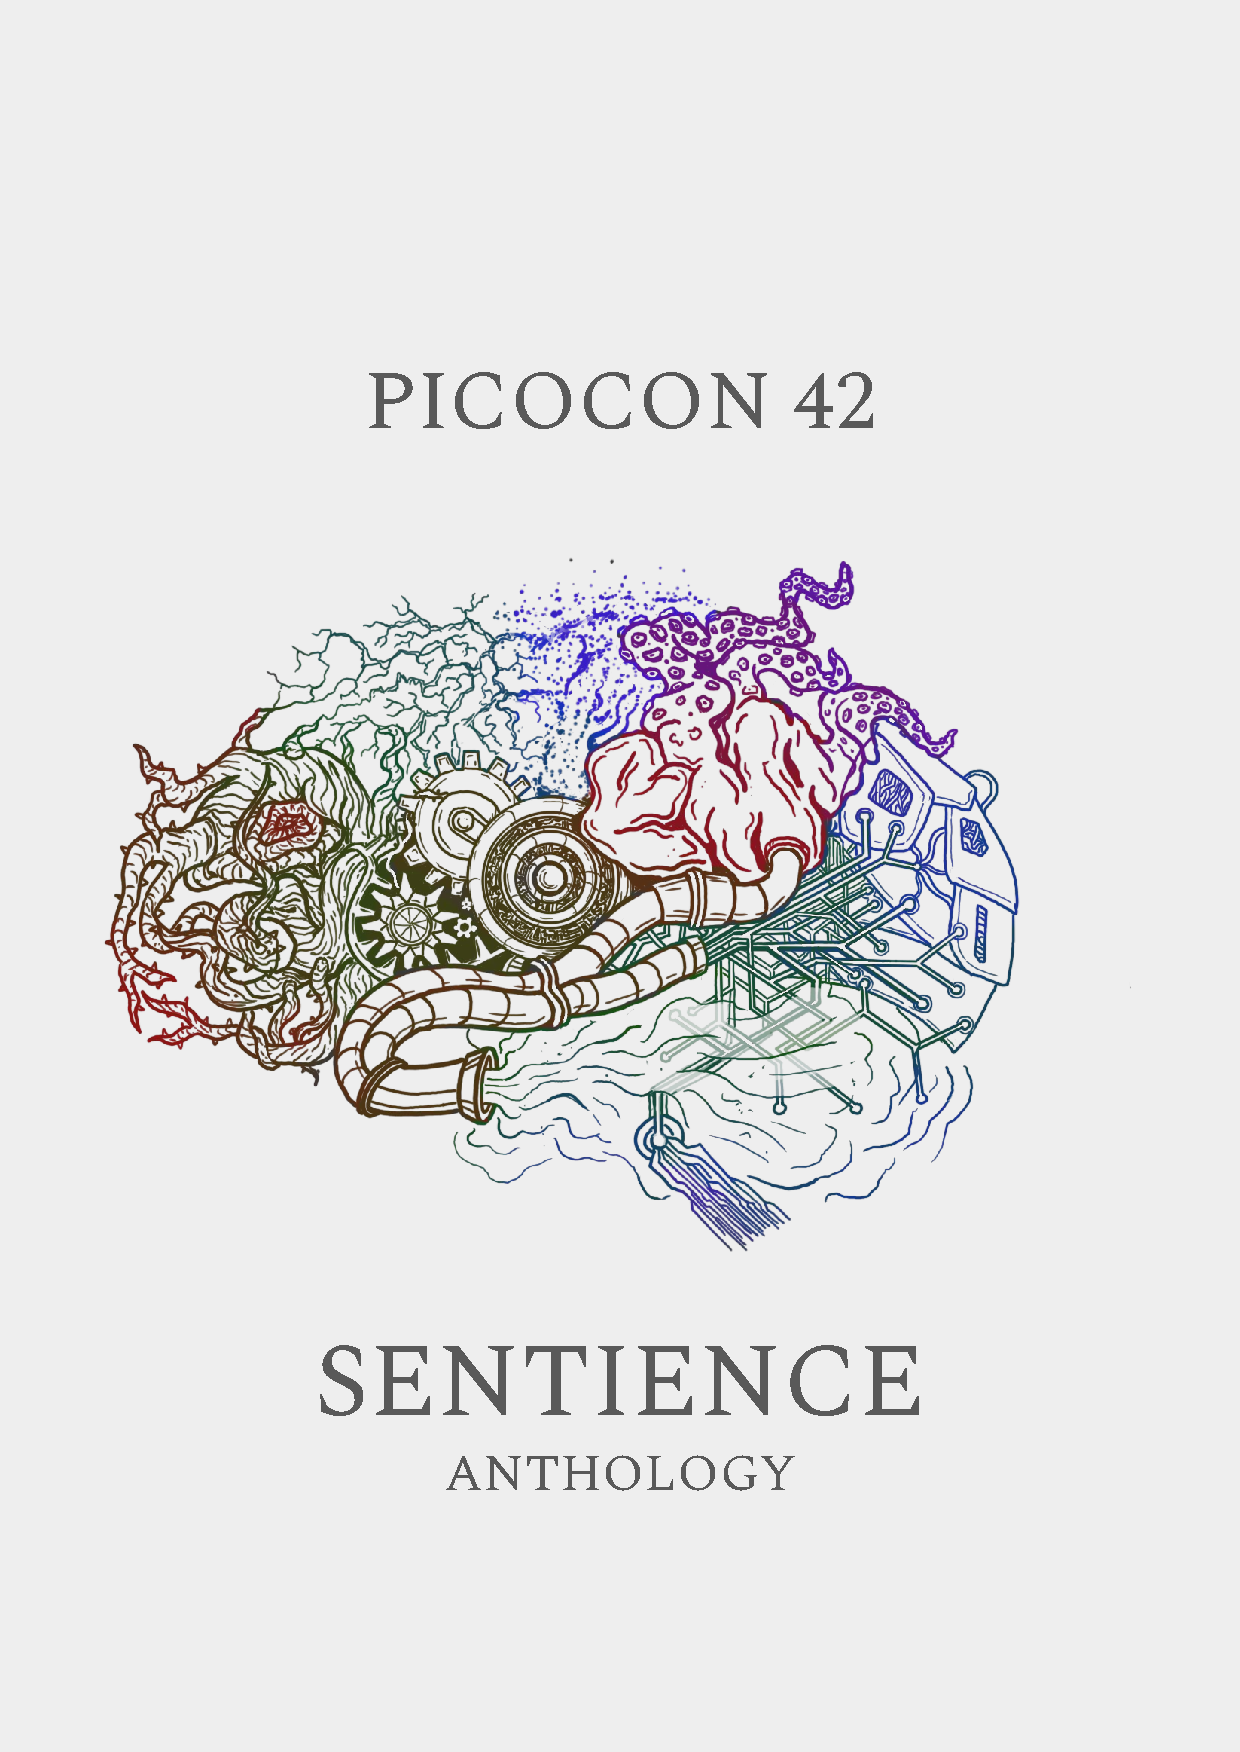
\includegraphics[width=\paperwidth,height=\paperheight]{img/sentience-cover.pdf}%
              }%
            }
            \vspace*{20cm}
            \color{white}
            \fontsize{25}{48}\selectfont 
\end{titlepage}
\begin{center}
    % \vspace*{10cm}
    \normalfont Credit to Rebecca Allday
\end{center}
\pagenumbering{roman}
\setcounter{page}{1}
\clearpage
\pagenumbering{arabic}
\setcounter{page}{1}
\head{Foreword}
Three years ago, I sat beside the previous Wyrmtongue Editor, the amazing Luke Conmy, to help edit the first Wyrmtongue short story collection in two years. It was called the “fanzine” then, and the world was only just recovering from the aftermath of a pandemic. It was only thanks to those who submitted to that first edition of Wyrmtongue (not a few who were committee members at the time) that the tradition of publishing a short story collection every year alongside Picocon was revived. It is with pride then, that I present to you the \textit{Wyrmtongue Anthology} series. 

I’m sure many in the committee will argue that this is just a rebranding of the old “fanzine”, but this is my corner, and fussing over semantics is my job, so I digress. While this is admittedly a bit of a self-indulgent title change, it is also part of a slow transition to make this series a little more “professional”, and also more work, much to the despair of the next editor in charge (sorry, Kai). As such, I really do hope you take the time to read these stories, because I sincerely believe that this batch contains some of the best I’ve read during my time as editor of \textit{Wyrmtongue}, and maybe it will convince you to submit something of your own in future editions of the \textit{Wyrmtongue Anthology}.

This edition begins with Jakub Dranczewski’s \textit{The Chinese Room}, named after John Searle’s philosophical argument on computer consciousness, or lack thereof. It is an interesting take on the concept, and I find it to be both a solid and appropriate opening for this year's theme of \textit{Sentience}. It is followed by \textit{The Rough} from Ruth Rafeeq, an incredible first year from WritSoc, and it is about a genetically engineered worker operating at a factory with less than stellar working conditions. 

The next two stories in this edition were written by myself and Juairiyah Raqib respectively -- both members of the current committee. \textit{The City} is a tale told through a logbook entry, about a traveler who finds themselves in a city with unusual properties; meanwhile, \textit{Artificial Idiocy} is a zany and humourous take on an everyman’s misplaced trust in artificial intelligence. 

The final story of this collection was written by a member of next year's committee -- Michael Porat-Bachmutsky tells the story of a sentient reindeer, who reminisces about their past during the twilight of their life.

That's all from me. I hope you enjoy this edition of the \textit{Wyrmtongue Anthology}, and happy reading! 
\tombstone

\hfill \parbox{0.3\textwidth}{{\large\textbf{\textemdash{} Clifford Chan}}\\\hspace*{1.7em}The Editor\\\hspace*{1.7em}February 2025}
\clearpage

\tableofcontents
\vfill
\clearpage

\story{The Chinese Room}{Jakub Dranczewski}{}{txt/chinese-room}
\vfill
\clearpage

\story{The Rough}{Ruth Rafeeq}{}{txt/the-rough}
\vfill
\clearpage

\story{The City}{Clifford Chan}{}{txt/the-city}
\vfill
\clearpage

\story{Artificial Idiocy}{Juairiyah Raqib}{}{txt/artificial-idiocy}
\vfill
\clearpage

\story{From the Perspective of a Philosophical Reindeer}{Michael 
Porat-Bachmutsky}{}{txt/deer}
\vfill
\clearpage
% how to make words not get cut like -?

% \poem{Kingmaker}{Aditi Mehendale}{txt/kingmaker}
% \vfill
% \clearpage

% \artpage{The Lady of Bloom}{Rebecca Allday}{img/the-lady-of-bloom-cropped}
% \vfill
% \clearpage

\text{ }
\clearpage

\text{ }
\clearpage

\text{ }
\pagenumbering{gobble}
\clearpage

\text{ }
\pagenumbering{gobble}
\AddToShipoutPictureBG*{%
              \AtPageLowerLeft{%
                
\includegraphics[width=\paperwidth,height=\paperheight]{img/wyrm-back.pdf}%
              }%
            }
\clearpage

% \clearpage
% \thispagestyle{empty}
% \vspace*{\fill}
% \begin{center}
  % 
\includegraphics[width=\paperwidth]{img/wyrm-back.pdf}
% \end{center}
\end{document}
